\model{A Diagram and A C++ Code Snippet} \\
  \begin{center}
    \small
    \begin{tabular}{p{2in}p{3in}}
      \begin{minipage}{2in}
        \centering\par\vskip 10pt
        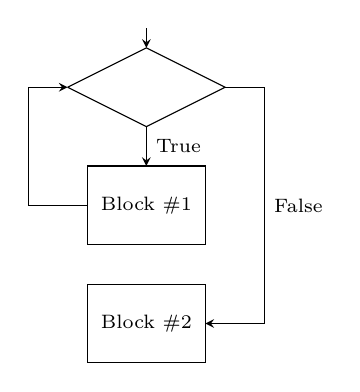
\begin{tikzpicture}
          % two rectangles
          \draw (0.25,1.5) -- (1.75,1.5) -- (1.75,2.5) -- (0.25,2.5) -- (0.25,1.5);
          \draw (0.25,0) -- (1.75,0) -- (1.75,1) -- (0.25,1) -- (0.25,0);
          % one triangle
          \draw (0,3.5) -- (1,3) -- (2,3.5) -- (1,4) -- (0,3.5);
          % five arrows
          \draw[-stealth] (1,4.25) -- (1,4);
          \draw[-stealth] (1,3) -- node[right] {\scriptsize True} (1,2.5);
          \draw[-stealth] (0.25,2) -- (-0.5,2) -- (-0.5,3.5) -- (0,3.5);
          \draw[-stealth] (2,3.5) -- (2.5,3.5) -- node[right] {\scriptsize False} (2.5,0.5) -- (1.75,0.5);
          % text
          \node[] at (1,2) {\scriptsize Block \#1};
          \node[] at (1,0.5) {\scriptsize Block \#2};
        \end{tikzpicture}
        \par\vskip 4pt\ \      
      \end{minipage}
      &
      \begin{minipage}{3in}
        \begin{cpplst}
#include <iostream>
#include <string>
using namespace std;

int main() {
  // print a person's name 10 times        
  string name;
  cout << "Enter your name: ";
  cin >> name;
  int x = 0;
  while (x < 10) {
    cout << name << endl;
    x = x + 1;
  }
  cout << "Nice to meet you!" << endl;
}
        \end{cpplst}
      \end{minipage}
    \end{tabular}
  \end{center}
  
  {\it\large Refer to Model 1 above as your team develops consensus answers
    to the questions below.}
    
  \quest{10 min}
  
  \Q Which lines of code go with the following shapes on the provided diagram?
    \begin{enumerate}
      \itemsep 10pt
      \item The diamond \hfill 
        \ans[4in]{Line 11 contains the condition in the diamond}

      \item The ``Block \#1'' rectangle \hfill 
        \ans[4in]{Lines 12 and 13 make up the statements if conditional is true \#1}

      \item The ``Block \#2'' rectangle \hfill 
        \ans[4in]{Line 15 contains the statement if conditional is false \#2}
    \end{enumerate}
    
  \Q Every loop structure requires three different actions.  Identify the line in the C++
    code snippet above that corresponds to each of these actions.
    \begin{enumerate}
      \itemsep 10pt
      \item {\bf Initialize} a variable to control the number of loop iterations. \hfill\ans[1in]{Line 10}
      \item {\bf Test} a condition to determine if we should keep looping. \hfill\ans[1in]{Line 11}
      \item {\bf Update} the variable involved in the test condition. \hfill\ans[1in]{Line 13}
    \end{enumerate}

  \Q The complete program is in {\tt activity07a.cpp}.  Run the program and
    answer the following questions.
    \begin{enumerate}
      \item What would the model program do differently if line 10 was: \cpp{int x = 1;}?
        \begin{answer}[0.4in]
          It would only print out 9 copies of the name.
        \end{answer}

      \item What would the model program do differently if line 11 was: \cpp{while (x <= 10)}?
        \begin{answer}[0.4in]          
          It would print out 11 copies of the name.
        \end{answer}

      \item What would the model program do differently if line 13 was: \cpp{x = x + 2;}?
        \begin{answer}[0.4in]
          It would only print out 5 copies of the name.
        \end{answer}
    \end{enumerate}
    \vskip -40pt
    
  \Q Change one or more of lines 11, 12, and 13 to make the program print the name 23 \key\\[-2.5mm] times.
    \begin{answer}[1.25in]
      \par
      Answers will vary, but one solution is to change line 10 to read:
      \begin{center}
        \cpp{ while ( x < 23 ) {}}
      \end{center}        
    \end{answer}